% !TeX root = ../praktikum.tex
% !TeX encoding = UTF-8
% !Tex spellcheck = de_DE
\begin{wrapfigure}{l}{7cm}
		\centering
		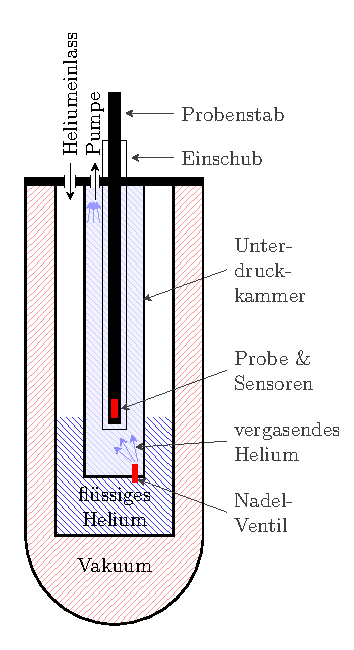
\includegraphics[scale=1]{graphs/aufbau/tank.pdf}
		\caption[Schematischer Aufbau des Kryostaten]{Schematische Zeichnung des im Text beschriebenen Kryostaten.}
		\label{fig:kryo}
\end{wrapfigure}

Der Versuchsaufbau besteht aus einem im Boden eingelassenen Kryostaten und einer sich in einem Rack befindlichen Steuerungs- und Messelektronik, welche mit Hilfe eines Computers gesteuert bzw. ausgelesen wird und deren Messdaten aufgezeichnet werden können. Der Kryostat ist ein Vakuumtank mit einer heliumgefüllten Kammer im Inneren. Darin befindet sich eine Kammer, in der wiederum ein Probeneinschub ist. Mit einer Pumpe wird der Druck in dieser Kammer auf wenigen Millibar gehalten. Durch die Verdunstungskälte kann die Innentemperatur, und so effektiv auch die Probentemperatur auf etwa \unit[1,5]{K} gehalten werden. Dieser Aufbau ist in Abbildung~\ref{fig:kryo} schematisch dargestellt. Durch einige Sensoren und eine Heizung kann die Temperatur anschließend sehr genau geregelt werden. Um die beiden Effekte letztendlich beobachten zu können, sind sehr hohe Magnetfelder von Nöten, hierfür werden zwei supraleitende Magnetspulen genutzt.\\

Vor dem Versuch wurde der Tank über den Heliumeinlass an der Oberseite mit flüssigem Helium gefüllt. Die Probe wurde an der Spitze des Probenstabes montiert und in den Probeneinschub eingeführt. Anschließend wurde die den Einschub umgebende Kammer mehrfach mit Hilfe eines Nadelventils mit Helium geflutet und anschließend wieder abgepumpt, um Luftreste zu entfernen und Vereisungen an Probe und Nadelventil zu vermeiden. Anschließend wurde bei laufender Pumpe eine Einstellung für die Heliumzufuhr (Nadelventil) gesucht, sodass sich in der Kammer der gewünschte Unterdruck und somit die sehr tiefen Temperaturen einstellen.\\

Im Nachfolgenden werden in den ersten beiden Abschnitten zwei unterschiedliche Messmethoden erprobt und in den Anschließenden werden Winkel, Temperatur und Elektronendichte verändert und die Folgen auf den Quanten-Hall Effekt und die Shubnikov-de Haas Oszillationen untersucht.